\documentclass{report}
\usepackage{graphicx}
\usepackage[portuguese]{babel}
\usepackage[utf8]{inputenc}
\usepackage{hyperref}
\usepackage{color}
\usepackage{enumerate}
\usepackage{alltt}
\usepackage{fancyvrb}
\usepackage{listings}
\usepackage{amsmath}
\DefineVerbatimEnvironment{code}{Verbatim}{fontsize=\footnotesize}

\lstset{
	basicstyle=\small,
	numbers=left,
	numberstyle=\tiny,
	numbersep=5pt,
	breaklines=true,
    frame=tB,
	mathescape=true,
	escapeinside={(*@}{@*)}
	}


\usepackage{xspace}

\parindent=0pt
\parskip=2pt

\setlength{\oddsidemargin}{-1cm}
\setlength{\textwidth}{18cm}
\setlength{\headsep}{-1cm}
\setlength{\textheight}{23cm}



\title{Processamento de Linguagens e Compiladores (3º ano de LCC)\\ \textbf{Pré-processador para HTML}\\ TP1\\ Grupo 9}
\author{Filipe Barbosa\\ A77252 \and  Hugo Ferreira\\ A78555 \and Nuno Morais\\ A77368 }
\date{\today}

\begin{document}

\maketitle

\begin{abstract}
Neste relatório serão apresentadas as ideias implementadas para criar um pré-processador de HTML através da ferramenta $Flex$. 
Também descrevemos as decisões tomadas e as dificuldades encontradas, bem como apresentamos algumas imagens relativas ao trabalho efetuado.
\end{abstract}

\tableofcontents

\section{Introduction}
Escrever um documento em HTML torna-se muito exaustivo, devido ao peso das "tags" que são inseridas para anotar o texto. Por exemplo, para colocar alguma coisa em negrito é necessário fazer:$ <b>$(texto que queremos a negrito)$</b>$. \\ 
Por isso existem pré-processadores de HTML que facilitam a tarefa da inserção dessas "tags", pois permitem ao utilizador usar anotações mais leves e mais simples. Depois, o pré-processador substitui a notação abreviada para a notação de HTML.\\ 
No trabalho construímos um pré-processador que ajuda a simplificar a escrita do código HTML. 



\chapter{Pré-Processador} \label{fi}
\section{Descrição do problema}\
Neste trabalho é necessário:
\begin{enumerate}[i)]
\item Criar marcas menos pesadas que são inseridas para anotar o texto.
\item Através do Flex construir o processador.
\item Passar um ficheiro através do pré-processador para $HTML$.
\end{enumerate}

\section{Especificação dos requisitos}

Os requesitos para este trabalho passam por investigar o pré-processador da linguagem Wiki e especificar uma linguagem com símbolos que facilitassem a escrita de formatação, listas de tópicos numerados e não-numerados e que não interferisse na passagem para HTML.
 
\section{Expressões regulares} 

As expressões regulares usadas foram:

\begin{enumerate}[i)]
\item $ \{$$neg$$\} $
\item $ \{$$fimneg$$\} $
\item $ \{$$it$$\} $
\item $ \{$$fimit$$\} $
\item $ \{$$un$$\} $
\item $ \{$$fimun$$\} $
\item $ \{$$h1$$\} $
\item $ \{$$h2$$\} $
\item $ \{$$h3$$\} $
\item $ \{$$h4$$\} $
\item $ \{$$h5$$\} $
\item $ \{$$h6$$\} $
\item $ \{$$fimh1$$\} $
\item $ \{$$fimh2$$\} $
\item $ \{$$fimh3$$\} $
\item $ \{$$fimh4$$\} $
\item $ \{$$fimh5$$\} $
\item $ \{$$fimh6$$\} $


\end{enumerate}

\chapter{Codificação e Testes}
\section{Problemas de implementação e Decisões Tomadas}
\subsection{Problemas de implementação}

Globalmente, não experenciamos muitos problemas de implementação. Numa fase inicial nós tivemos alguns problemas porque não sabiamos quando as nossas implementações terminavam.   


\subsection{Decisões Tomadas}
Neste trabalho tivemos de escolher algumas marcas menos pesadas.\\ 
Para abreviar a escrita de formatação usamos: 

\begin{enumerate}[1-] 

\item Negrito: $\{$$neg$$\}(texto)\{$$fimneg$$\}$

\item Itálico: $\{$$it$$\}(texto)\{$$fimit$$\}$ 

\item Sublinhado: $\{$$un$$\}(texto)\{$$fimun$$\}$ 

\item Níveis de títulos: $\{$$h[1-6]$$\}(texto)\{$$fimh[1-6]$$\}$ 

\item Listas não numeradas: $\{$$ul$$\}[item | item|... ]\{$$fimul$$\}$ 

\item Listas numeradas: $\{$$ol$$\}[item | item|... ]\{$$fimol$$\}$


\end{enumerate}
Caso alguém queira utilizar algum dos símbolos, mas não usar a sua formatação, basta acrescentar um $\{neg\}$ 
antes dos símbolos e depois dos simbolos um $\{fimneg\}$. Por exemplo escrever a expressão matemática "$3>1$" em negrito, basta fazer  " $\{$$neg$$\}3>1\{$$fimneg$$\}$" 



\section{Testes realizados e Resultados}

Criamos um ficheiro txt com as nossas anotações mais simples e mais leves. (Figura A.1). Depois através do ficheiro makefile, compilamos o nosso ficheiro em $Flex$ e passamos ao executável o ficheiro txt (Figura A.2 e A.3).\\ 
Como resultado obtemos um ficheiro já com as anotações do HTML (Figura A.4).
Por fim temos o exemplo HTML (Figura A.5).



\chapter{Conclusão} \label{concl}

Nos tempos que correm já se encontram disponiveis muitos pré-processadores que facilitam a escrita de documentos em HTML.\\
Tendo em conta os aspetos apresentados no decorrer do nosso relatório, conclui-se que o $Flex$ é uma ferramenta simples e eficiente para fazer o pré-processador e que com ele se torna fácil programar usando expressões regulares e um pouco de linguagem C. \\
Futuramente poderíamos acrescentar mais simbolos e implementar dicionários para completar o pré processador.


\appendix
\chapter{Figuras}
\begin{figure}[ht]
\centering
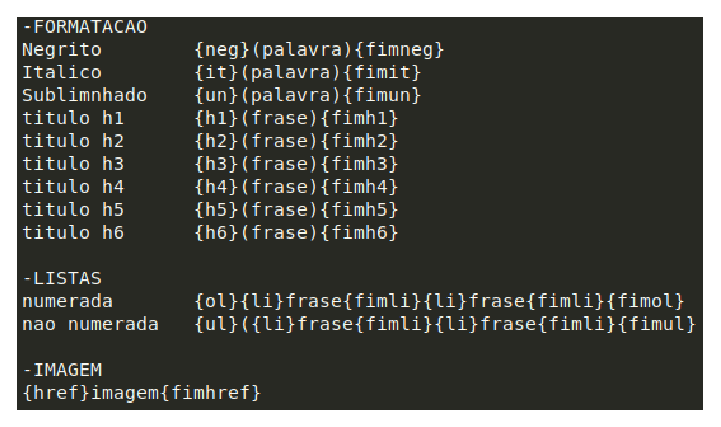
\includegraphics[width=12cm,height=10cm]{linguagem.eps}
\caption{Exemplo com as "tags" simplificadas}
\label{Exemplo 1}
\end{figure}

\begin{figure}[ht]
\centering
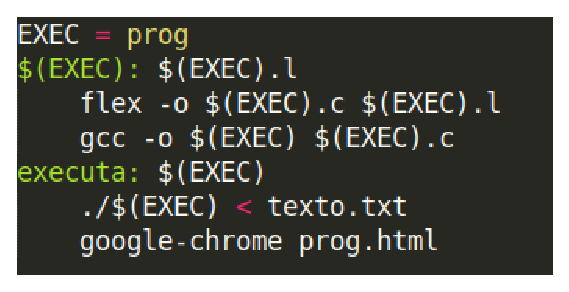
\includegraphics[width=7cm,height=2cm]{makefile.eps}
\caption{Ficheiro makefile}
\label{makefile}
\end{figure}

\begin{figure}[ht]
\centering
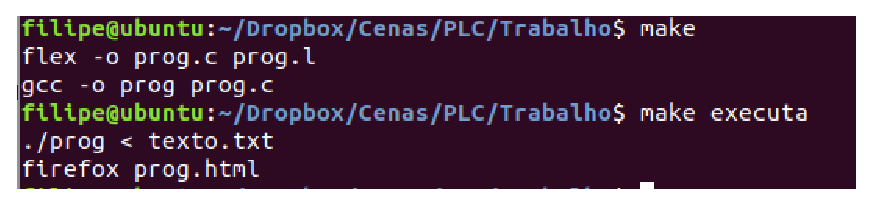
\includegraphics[width=12cm,height=2cm]{cmd.eps}
\caption{Terminal}
\label{Terminal}
\end{figure}

\begin{figure}[ht]
\centering
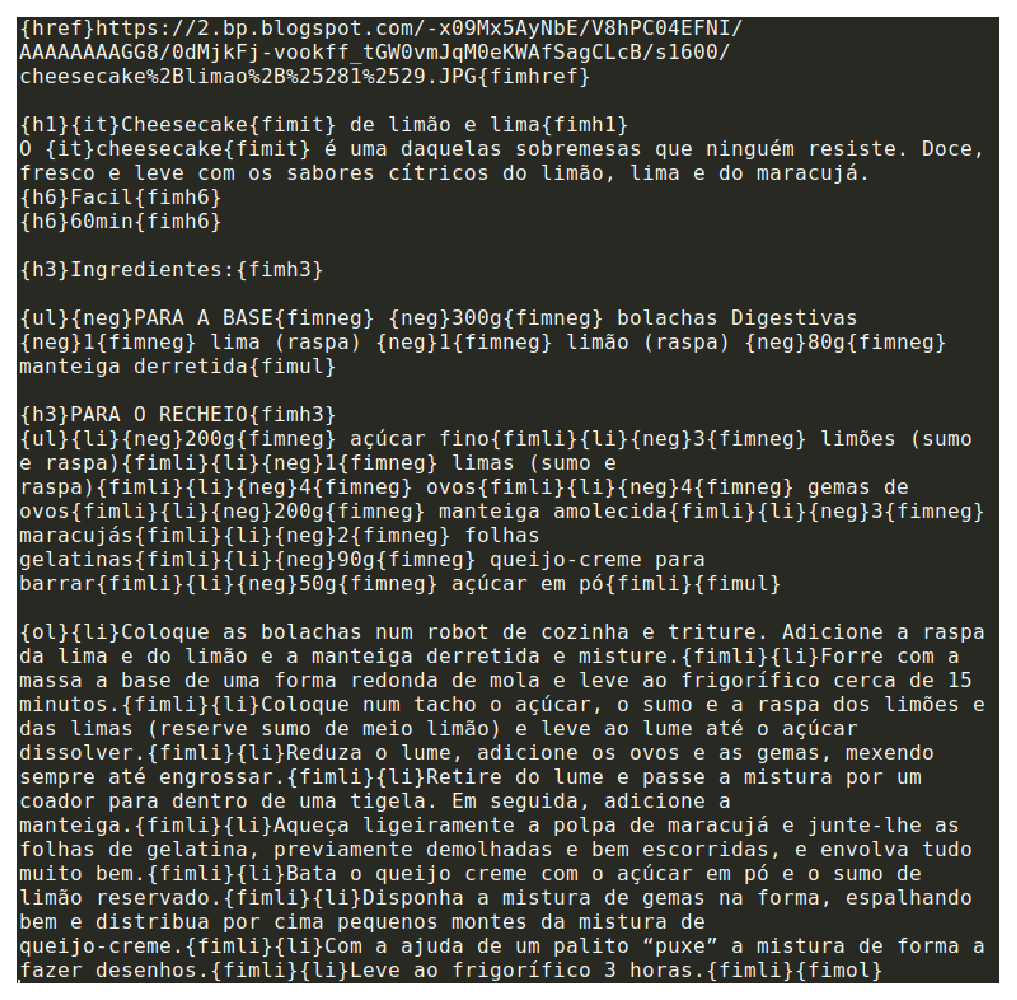
\includegraphics[width=9cm,height=9cm]{texto.eps}
\caption{Exemplo de texto}
\label{Ficheiro em txt}
\end{figure}

\begin{figure}[ht]
\centering
\includegraphics[width=9cm,height=9cm]{HTML.eps}
\caption{Exemplo HTML}
\label{HTML}
\end{figure}


\chapter{Código do Pré-Processador}

\begin{code}

%{
#include <stdlib.h>
#include <stdio.h>
#include <string.h>
FILE* f;
%}

%x cmd

%%
\{it\} {fprintf(f,"<i>"); }
\{fimit\} {fprintf(f,"</i>"); }
\{neg\} {fprintf(f,"<b>"); }
\{fimneg\} {fprintf(f,"</b>"); }
\{un\} {fprintf(f,"<u>"); }
\{fimun\} {fprintf(f,"</u>"); }
\{h1\} {fprintf(f,"<h1>"); }
\{fimh1\} {fprintf(f,"</h1>"); }
\{h2\} {fprintf(f,"<h2>"); }
\{fimh2\} {fprintf(f,"</h2>"); }
\{h3\} {fprintf(f,"<h3>"); }
\{fimh3\} {fprintf(f,"</h3>"); }
\{h4\} {fprintf(f,"<h4>"); }
\{fimh4\} {fprintf(f,"</h4>"); }
\{h5\} {fprintf(f,"<h5>"); }
\{fimh5\} {fprintf(f,"</h5>"); }
\{h6\} {fprintf(f,"<h6>"); }
\{fimh6\} {fprintf(f,"</h6>"); }
\{ol\} {fprintf(f,"<ol>"); }
\{fimol\} {fprintf(f,"</ol>"); }
\{ul\} {fprintf(f,"<ul>"); }
\{fimul\} {fprintf(f,"</ul>"); }
\{li\} {fprintf(f,"<li>"); }
\{fimli\} {fprintf(f,"</li>"); }
\{href\} {fprintf(f,"<img src="); }
\{fimhref\} {fprintf(f," height=150>"); }
(.|\n) {fprintf(f,"%s",yytext); }

%%

void printheader(){
	fprintf(f,"<!DOCTYPE html>\n");
	fprintf(f,"<html lang=%cpt%c>\n",34,34);
	fprintf(f,"<head>\n");
	fprintf(f,"<meta charset=%cutf-8%c>\n",34,34);
	fprintf(f,"</head>\n");
	fprintf(f,"<body>\n");
}



int yywrap(){
	return (1);
}

int main(){
	f=fopen("prog.html","w");
	printheader();
	yylex();
	fprintf(f,"</body>\n");
	fprintf(f,"</html>\n");
	fclose(f);
	return 0;
}
\end{code}


\end{document}
